\documentclass{article}

\usepackage{iclr2027_conference,times}
%%%%% NEW MATH DEFINITIONS %%%%%

\usepackage{amsmath,amsfonts,bm}

% Mark sections of captions for referring to divisions of figures
\newcommand{\figleft}{{\em (Left)}}
\newcommand{\figcenter}{{\em (Center)}}
\newcommand{\figright}{{\em (Right)}}
\newcommand{\figtop}{{\em (Top)}}
\newcommand{\figbottom}{{\em (Bottom)}}
\newcommand{\captiona}{{\em (a)}}
\newcommand{\captionb}{{\em (b)}}
\newcommand{\captionc}{{\em (c)}}
\newcommand{\captiond}{{\em (d)}}

% Highlight a newly defined term
\newcommand{\newterm}[1]{{\bf #1}}


% Figure reference, lower-case.
\def\figref#1{figure~\ref{#1}}
% Figure reference, capital. For start of sentence
\def\Figref#1{Figure~\ref{#1}}
\def\twofigref#1#2{figures \ref{#1} and \ref{#2}}
\def\quadfigref#1#2#3#4{figures \ref{#1}, \ref{#2}, \ref{#3} and \ref{#4}}
% Section reference, lower-case.
\def\secref#1{section~\ref{#1}}
% Section reference, capital.
\def\Secref#1{Section~\ref{#1}}
% Reference to two sections.
\def\twosecrefs#1#2{sections \ref{#1} and \ref{#2}}
% Reference to three sections.
\def\secrefs#1#2#3{sections \ref{#1}, \ref{#2} and \ref{#3}}
% Reference to an equation, lower-case.
\def\eqref#1{equation~\ref{#1}}
% Reference to an equation, upper case
\def\Eqref#1{Equation~\ref{#1}}
% A raw reference to an equation---avoid using if possible
\def\plaineqref#1{\ref{#1}}
% Reference to a chapter, lower-case.
\def\chapref#1{chapter~\ref{#1}}
% Reference to an equation, upper case.
\def\Chapref#1{Chapter~\ref{#1}}
% Reference to a range of chapters
\def\rangechapref#1#2{chapters\ref{#1}--\ref{#2}}
% Reference to an algorithm, lower-case.
\def\algref#1{algorithm~\ref{#1}}
% Reference to an algorithm, upper case.
\def\Algref#1{Algorithm~\ref{#1}}
\def\twoalgref#1#2{algorithms \ref{#1} and \ref{#2}}
\def\Twoalgref#1#2{Algorithms \ref{#1} and \ref{#2}}
% Reference to a part, lower case
\def\partref#1{part~\ref{#1}}
% Reference to a part, upper case
\def\Partref#1{Part~\ref{#1}}
\def\twopartref#1#2{parts \ref{#1} and \ref{#2}}

\def\ceil#1{\lceil #1 \rceil}
\def\floor#1{\lfloor #1 \rfloor}
\def\1{\bm{1}}
\newcommand{\train}{\mathcal{D}}
\newcommand{\valid}{\mathcal{D_{\mathrm{valid}}}}
\newcommand{\test}{\mathcal{D_{\mathrm{test}}}}

\def\eps{{\epsilon}}


% Random variables
\def\reta{{\textnormal{$\eta$}}}
\def\ra{{\textnormal{a}}}
\def\rb{{\textnormal{b}}}
\def\rc{{\textnormal{c}}}
\def\rd{{\textnormal{d}}}
\def\re{{\textnormal{e}}}
\def\rf{{\textnormal{f}}}
\def\rg{{\textnormal{g}}}
\def\rh{{\textnormal{h}}}
\def\ri{{\textnormal{i}}}
\def\rj{{\textnormal{j}}}
\def\rk{{\textnormal{k}}}
\def\rl{{\textnormal{l}}}
% rm is already a command, just don't name any random variables m
\def\rn{{\textnormal{n}}}
\def\ro{{\textnormal{o}}}
\def\rp{{\textnormal{p}}}
\def\rq{{\textnormal{q}}}
\def\rr{{\textnormal{r}}}
\def\rs{{\textnormal{s}}}
\def\rt{{\textnormal{t}}}
\def\ru{{\textnormal{u}}}
\def\rv{{\textnormal{v}}}
\def\rw{{\textnormal{w}}}
\def\rx{{\textnormal{x}}}
\def\ry{{\textnormal{y}}}
\def\rz{{\textnormal{z}}}

% Random vectors
\def\rvepsilon{{\mathbf{\epsilon}}}
\def\rvtheta{{\mathbf{\theta}}}
\def\rva{{\mathbf{a}}}
\def\rvb{{\mathbf{b}}}
\def\rvc{{\mathbf{c}}}
\def\rvd{{\mathbf{d}}}
\def\rve{{\mathbf{e}}}
\def\rvf{{\mathbf{f}}}
\def\rvg{{\mathbf{g}}}
\def\rvh{{\mathbf{h}}}
\def\rvu{{\mathbf{i}}}
\def\rvj{{\mathbf{j}}}
\def\rvk{{\mathbf{k}}}
\def\rvl{{\mathbf{l}}}
\def\rvm{{\mathbf{m}}}
\def\rvn{{\mathbf{n}}}
\def\rvo{{\mathbf{o}}}
\def\rvp{{\mathbf{p}}}
\def\rvq{{\mathbf{q}}}
\def\rvr{{\mathbf{r}}}
\def\rvs{{\mathbf{s}}}
\def\rvt{{\mathbf{t}}}
\def\rvu{{\mathbf{u}}}
\def\rvv{{\mathbf{v}}}
\def\rvw{{\mathbf{w}}}
\def\rvx{{\mathbf{x}}}
\def\rvy{{\mathbf{y}}}
\def\rvz{{\mathbf{z}}}

% Elements of random vectors
\def\erva{{\textnormal{a}}}
\def\ervb{{\textnormal{b}}}
\def\ervc{{\textnormal{c}}}
\def\ervd{{\textnormal{d}}}
\def\erve{{\textnormal{e}}}
\def\ervf{{\textnormal{f}}}
\def\ervg{{\textnormal{g}}}
\def\ervh{{\textnormal{h}}}
\def\ervi{{\textnormal{i}}}
\def\ervj{{\textnormal{j}}}
\def\ervk{{\textnormal{k}}}
\def\ervl{{\textnormal{l}}}
\def\ervm{{\textnormal{m}}}
\def\ervn{{\textnormal{n}}}
\def\ervo{{\textnormal{o}}}
\def\ervp{{\textnormal{p}}}
\def\ervq{{\textnormal{q}}}
\def\ervr{{\textnormal{r}}}
\def\ervs{{\textnormal{s}}}
\def\ervt{{\textnormal{t}}}
\def\ervu{{\textnormal{u}}}
\def\ervv{{\textnormal{v}}}
\def\ervw{{\textnormal{w}}}
\def\ervx{{\textnormal{x}}}
\def\ervy{{\textnormal{y}}}
\def\ervz{{\textnormal{z}}}

% Random matrices
\def\rmA{{\mathbf{A}}}
\def\rmB{{\mathbf{B}}}
\def\rmC{{\mathbf{C}}}
\def\rmD{{\mathbf{D}}}
\def\rmE{{\mathbf{E}}}
\def\rmF{{\mathbf{F}}}
\def\rmG{{\mathbf{G}}}
\def\rmH{{\mathbf{H}}}
\def\rmI{{\mathbf{I}}}
\def\rmJ{{\mathbf{J}}}
\def\rmK{{\mathbf{K}}}
\def\rmL{{\mathbf{L}}}
\def\rmM{{\mathbf{M}}}
\def\rmN{{\mathbf{N}}}
\def\rmO{{\mathbf{O}}}
\def\rmP{{\mathbf{P}}}
\def\rmQ{{\mathbf{Q}}}
\def\rmR{{\mathbf{R}}}
\def\rmS{{\mathbf{S}}}
\def\rmT{{\mathbf{T}}}
\def\rmU{{\mathbf{U}}}
\def\rmV{{\mathbf{V}}}
\def\rmW{{\mathbf{W}}}
\def\rmX{{\mathbf{X}}}
\def\rmY{{\mathbf{Y}}}
\def\rmZ{{\mathbf{Z}}}

% Elements of random matrices
\def\ermA{{\textnormal{A}}}
\def\ermB{{\textnormal{B}}}
\def\ermC{{\textnormal{C}}}
\def\ermD{{\textnormal{D}}}
\def\ermE{{\textnormal{E}}}
\def\ermF{{\textnormal{F}}}
\def\ermG{{\textnormal{G}}}
\def\ermH{{\textnormal{H}}}
\def\ermI{{\textnormal{I}}}
\def\ermJ{{\textnormal{J}}}
\def\ermK{{\textnormal{K}}}
\def\ermL{{\textnormal{L}}}
\def\ermM{{\textnormal{M}}}
\def\ermN{{\textnormal{N}}}
\def\ermO{{\textnormal{O}}}
\def\ermP{{\textnormal{P}}}
\def\ermQ{{\textnormal{Q}}}
\def\ermR{{\textnormal{R}}}
\def\ermS{{\textnormal{S}}}
\def\ermT{{\textnormal{T}}}
\def\ermU{{\textnormal{U}}}
\def\ermV{{\textnormal{V}}}
\def\ermW{{\textnormal{W}}}
\def\ermX{{\textnormal{X}}}
\def\ermY{{\textnormal{Y}}}
\def\ermZ{{\textnormal{Z}}}

% Vectors
\def\vzero{{\bm{0}}}
\def\vone{{\bm{1}}}
\def\vmu{{\bm{\mu}}}
\def\vtheta{{\bm{\theta}}}
\def\va{{\bm{a}}}
\def\vb{{\bm{b}}}
\def\vc{{\bm{c}}}
\def\vd{{\bm{d}}}
\def\ve{{\bm{e}}}
\def\vf{{\bm{f}}}
\def\vg{{\bm{g}}}
\def\vh{{\bm{h}}}
\def\vi{{\bm{i}}}
\def\vj{{\bm{j}}}
\def\vk{{\bm{k}}}
\def\vl{{\bm{l}}}
\def\vm{{\bm{m}}}
\def\vn{{\bm{n}}}
\def\vo{{\bm{o}}}
\def\vp{{\bm{p}}}
\def\vq{{\bm{q}}}
\def\vr{{\bm{r}}}
\def\vs{{\bm{s}}}
\def\vt{{\bm{t}}}
\def\vu{{\bm{u}}}
\def\vv{{\bm{v}}}
\def\vw{{\bm{w}}}
\def\vx{{\bm{x}}}
\def\vy{{\bm{y}}}
\def\vz{{\bm{z}}}

% Elements of vectors
\def\evalpha{{\alpha}}
\def\evbeta{{\beta}}
\def\evepsilon{{\epsilon}}
\def\evlambda{{\lambda}}
\def\evomega{{\omega}}
\def\evmu{{\mu}}
\def\evpsi{{\psi}}
\def\evsigma{{\sigma}}
\def\evtheta{{\theta}}
\def\eva{{a}}
\def\evb{{b}}
\def\evc{{c}}
\def\evd{{d}}
\def\eve{{e}}
\def\evf{{f}}
\def\evg{{g}}
\def\evh{{h}}
\def\evi{{i}}
\def\evj{{j}}
\def\evk{{k}}
\def\evl{{l}}
\def\evm{{m}}
\def\evn{{n}}
\def\evo{{o}}
\def\evp{{p}}
\def\evq{{q}}
\def\evr{{r}}
\def\evs{{s}}
\def\evt{{t}}
\def\evu{{u}}
\def\evv{{v}}
\def\evw{{w}}
\def\evx{{x}}
\def\evy{{y}}
\def\evz{{z}}

% Matrix
\def\mA{{\bm{A}}}
\def\mB{{\bm{B}}}
\def\mC{{\bm{C}}}
\def\mD{{\bm{D}}}
\def\mE{{\bm{E}}}
\def\mF{{\bm{F}}}
\def\mG{{\bm{G}}}
\def\mH{{\bm{H}}}
\def\mI{{\bm{I}}}
\def\mJ{{\bm{J}}}
\def\mK{{\bm{K}}}
\def\mL{{\bm{L}}}
\def\mM{{\bm{M}}}
\def\mN{{\bm{N}}}
\def\mO{{\bm{O}}}
\def\mP{{\bm{P}}}
\def\mQ{{\bm{Q}}}
\def\mR{{\bm{R}}}
\def\mS{{\bm{S}}}
\def\mT{{\bm{T}}}
\def\mU{{\bm{U}}}
\def\mV{{\bm{V}}}
\def\mW{{\bm{W}}}
\def\mX{{\bm{X}}}
\def\mY{{\bm{Y}}}
\def\mZ{{\bm{Z}}}
\def\mBeta{{\bm{\beta}}}
\def\mPhi{{\bm{\Phi}}}
\def\mLambda{{\bm{\Lambda}}}
\def\mSigma{{\bm{\Sigma}}}

% Tensor
\DeclareMathAlphabet{\mathsfit}{\encodingdefault}{\sfdefault}{m}{sl}
\SetMathAlphabet{\mathsfit}{bold}{\encodingdefault}{\sfdefault}{bx}{n}
\newcommand{\tens}[1]{\bm{\mathsfit{#1}}}
\def\tA{{\tens{A}}}
\def\tB{{\tens{B}}}
\def\tC{{\tens{C}}}
\def\tD{{\tens{D}}}
\def\tE{{\tens{E}}}
\def\tF{{\tens{F}}}
\def\tG{{\tens{G}}}
\def\tH{{\tens{H}}}
\def\tI{{\tens{I}}}
\def\tJ{{\tens{J}}}
\def\tK{{\tens{K}}}
\def\tL{{\tens{L}}}
\def\tM{{\tens{M}}}
\def\tN{{\tens{N}}}
\def\tO{{\tens{O}}}
\def\tP{{\tens{P}}}
\def\tQ{{\tens{Q}}}
\def\tR{{\tens{R}}}
\def\tS{{\tens{S}}}
\def\tT{{\tens{T}}}
\def\tU{{\tens{U}}}
\def\tV{{\tens{V}}}
\def\tW{{\tens{W}}}
\def\tX{{\tens{X}}}
\def\tY{{\tens{Y}}}
\def\tZ{{\tens{Z}}}


% Graph
\def\gA{{\mathcal{A}}}
\def\gB{{\mathcal{B}}}
\def\gC{{\mathcal{C}}}
\def\gD{{\mathcal{D}}}
\def\gE{{\mathcal{E}}}
\def\gF{{\mathcal{F}}}
\def\gG{{\mathcal{G}}}
\def\gH{{\mathcal{H}}}
\def\gI{{\mathcal{I}}}
\def\gJ{{\mathcal{J}}}
\def\gK{{\mathcal{K}}}
\def\gL{{\mathcal{L}}}
\def\gM{{\mathcal{M}}}
\def\gN{{\mathcal{N}}}
\def\gO{{\mathcal{O}}}
\def\gP{{\mathcal{P}}}
\def\gQ{{\mathcal{Q}}}
\def\gR{{\mathcal{R}}}
\def\gS{{\mathcal{S}}}
\def\gT{{\mathcal{T}}}
\def\gU{{\mathcal{U}}}
\def\gV{{\mathcal{V}}}
\def\gW{{\mathcal{W}}}
\def\gX{{\mathcal{X}}}
\def\gY{{\mathcal{Y}}}
\def\gZ{{\mathcal{Z}}}

% Sets
\def\sA{{\mathbb{A}}}
\def\sB{{\mathbb{B}}}
\def\sC{{\mathbb{C}}}
\def\sD{{\mathbb{D}}}
% Don't use a set called E, because this would be the same as our symbol
% for expectation.
\def\sF{{\mathbb{F}}}
\def\sG{{\mathbb{G}}}
\def\sH{{\mathbb{H}}}
\def\sI{{\mathbb{I}}}
\def\sJ{{\mathbb{J}}}
\def\sK{{\mathbb{K}}}
\def\sL{{\mathbb{L}}}
\def\sM{{\mathbb{M}}}
\def\sN{{\mathbb{N}}}
\def\sO{{\mathbb{O}}}
\def\sP{{\mathbb{P}}}
\def\sQ{{\mathbb{Q}}}
\def\sR{{\mathbb{R}}}
\def\sS{{\mathbb{S}}}
\def\sT{{\mathbb{T}}}
\def\sU{{\mathbb{U}}}
\def\sV{{\mathbb{V}}}
\def\sW{{\mathbb{W}}}
\def\sX{{\mathbb{X}}}
\def\sY{{\mathbb{Y}}}
\def\sZ{{\mathbb{Z}}}

% Entries of a matrix
\def\emLambda{{\Lambda}}
\def\emA{{A}}
\def\emB{{B}}
\def\emC{{C}}
\def\emD{{D}}
\def\emE{{E}}
\def\emF{{F}}
\def\emG{{G}}
\def\emH{{H}}
\def\emI{{I}}
\def\emJ{{J}}
\def\emK{{K}}
\def\emL{{L}}
\def\emM{{M}}
\def\emN{{N}}
\def\emO{{O}}
\def\emP{{P}}
\def\emQ{{Q}}
\def\emR{{R}}
\def\emS{{S}}
\def\emT{{T}}
\def\emU{{U}}
\def\emV{{V}}
\def\emW{{W}}
\def\emX{{X}}
\def\emY{{Y}}
\def\emZ{{Z}}
\def\emSigma{{\Sigma}}

% entries of a tensor
% Same font as tensor, without \bm wrapper
\newcommand{\etens}[1]{\mathsfit{#1}}
\def\etLambda{{\etens{\Lambda}}}
\def\etA{{\etens{A}}}
\def\etB{{\etens{B}}}
\def\etC{{\etens{C}}}
\def\etD{{\etens{D}}}
\def\etE{{\etens{E}}}
\def\etF{{\etens{F}}}
\def\etG{{\etens{G}}}
\def\etH{{\etens{H}}}
\def\etI{{\etens{I}}}
\def\etJ{{\etens{J}}}
\def\etK{{\etens{K}}}
\def\etL{{\etens{L}}}
\def\etM{{\etens{M}}}
\def\etN{{\etens{N}}}
\def\etO{{\etens{O}}}
\def\etP{{\etens{P}}}
\def\etQ{{\etens{Q}}}
\def\etR{{\etens{R}}}
\def\etS{{\etens{S}}}
\def\etT{{\etens{T}}}
\def\etU{{\etens{U}}}
\def\etV{{\etens{V}}}
\def\etW{{\etens{W}}}
\def\etX{{\etens{X}}}
\def\etY{{\etens{Y}}}
\def\etZ{{\etens{Z}}}

% The true underlying data generating distribution
\newcommand{\pdata}{p_{\rm{data}}}
% The empirical distribution defined by the training set
\newcommand{\ptrain}{\hat{p}_{\rm{data}}}
\newcommand{\Ptrain}{\hat{P}_{\rm{data}}}
% The model distribution
\newcommand{\pmodel}{p_{\rm{model}}}
\newcommand{\Pmodel}{P_{\rm{model}}}
\newcommand{\ptildemodel}{\tilde{p}_{\rm{model}}}
% Stochastic autoencoder distributions
\newcommand{\pencode}{p_{\rm{encoder}}}
\newcommand{\pdecode}{p_{\rm{decoder}}}
\newcommand{\precons}{p_{\rm{reconstruct}}}

\newcommand{\laplace}{\mathrm{Laplace}} % Laplace distribution

\newcommand{\E}{\mathbb{E}}
\newcommand{\Ls}{\mathcal{L}}
\newcommand{\R}{\mathbb{R}}
\newcommand{\emp}{\tilde{p}}
\newcommand{\lr}{\alpha}
\newcommand{\reg}{\lambda}
\newcommand{\rect}{\mathrm{rectifier}}
\newcommand{\softmax}{\mathrm{softmax}}
\newcommand{\sigmoid}{\sigma}
\newcommand{\softplus}{\zeta}
\newcommand{\KL}{D_{\mathrm{KL}}}
\newcommand{\Var}{\mathrm{Var}}
\newcommand{\standarderror}{\mathrm{SE}}
\newcommand{\Cov}{\mathrm{Cov}}
% Wolfram Mathworld says $L^2$ is for function spaces and $\ell^2$ is for vectors
% But then they seem to use $L^2$ for vectors throughout the site, and so does
% wikipedia.
\newcommand{\normlzero}{L^0}
\newcommand{\normlone}{L^1}
\newcommand{\normltwo}{L^2}
\newcommand{\normlp}{L^p}
\newcommand{\normmax}{L^\infty}

\newcommand{\parents}{Pa} % See usage in notation.tex. Chosen to match Daphne's book.

\DeclareMathOperator*{\argmax}{arg\,max}
\DeclareMathOperator*{\argmin}{arg\,min}

\DeclareMathOperator{\sign}{sign}
\DeclareMathOperator{\Tr}{Tr}
\let\ab\allowbreak


\usepackage{hyperref}
\usepackage{url}
\usepackage{graphicx}
\usepackage{amsmath,amssymb,bm}
\usepackage{booktabs,array,multirow,threeparttable,adjustbox}
\usepackage{tikz}
\usetikzlibrary{arrows.meta,positioning,fit,calc}
\hypersetup{hidelinks}

\title{RAL-MoE-ROM: Hierarchical Mixture-of-Experts for Regime-Adaptive Reduced Dynamics}

% Anonymous submission. Restore the author block only for the camera-ready version.
\author{Anonymous Authors}

% Keep disabled for the anonymous submission.
% \iclrfinalcopy

\begin{document}

\maketitle

\begin{abstract}
Learning reduced dynamical models over broad parameter ranges is challenging when the underlying system exhibits qualitatively different regimes. A single global representation must simultaneously encode distinct local state geometries, while a single learned dynamical model must reproduce different stability, growth, and saturation mechanisms under recursive rollout. We introduce RAL-MoE-ROM, a two-level hierarchical mixture-of-experts framework for regime-adaptive reduced dynamics. The parameterized solution set is represented by overlapping regime-local reduced charts, each equipped with an autonomous physics--data specialist. Within each specialist, a structured sparse mixture of experts learns corrections to the projected reduced dynamics using nonlinear, affine, and low-rank bilinear expert branches selected by hierarchical sparse routing. A second routing level operates across regime-local specialists. Because the local charts have independent reduced coordinates, adjacent specialists are advanced independently and combined only after reconstruction in the common physical space through a learned Top-2 convex correction. Across three parametrized incompressible-flow benchmarks spanning steady, Hopf-onset, and periodic dynamics, the proposed specialists provide accurate long-horizon autonomous predictions, while the hierarchical fusion consistently improves predictions in evaluated transition regions. Ablations further show complementary contributions from structured expert specialization, the projected physical backbone, regime localization, and learned cross-regime routing.
\end{abstract}

\section{Introduction}

Learning compact dynamical models is central to scientific machine learning when
high-fidelity simulations are too expensive to evaluate repeatedly.
The challenge becomes substantially harder when a physical parameter changes not only the
magnitude of the response, but also the qualitative character of the dynamics.
Parameterized incompressible flows provide a representative example: different portions of
the parameter domain may exhibit relaxation toward a steady state, weak oscillatory growth
near instability onset, or sustained nonlinear periodic motion.
A reduced model intended for many-query prediction must therefore remain accurate under
autonomous rollout while the underlying dynamics vary across qualitatively different
regimes.

This setting exposes two coupled difficulties.
First, the state representation itself can be strongly regime dependent.
A low-dimensional basis that efficiently describes nearly steady states need not provide an
equally compact description of developed periodic dynamics.
Second, even when a suitable reduced representation is available, the corresponding
dynamical model must reproduce different temporal mechanisms, including decay, growth,
phase evolution, and nonlinear saturation.
A single global reduced model must solve both problems simultaneously: it must encode
states drawn from distinct local geometries and learn a dynamical law that remains accurate
over all of them.
This requirement is particularly demanding for autonomous prediction, where small local
errors are recursively propagated over long horizons.

Projection-based reduced-order models provide an explicit low-dimensional dynamical
structure through methods such as proper orthogonal decomposition (POD) and Galerkin
projection \citep{sirovich1987,berkooz1993,benner2015}.
Their predictive accuracy, however, can deteriorate when truncated modes contribute to
dissipation, nonlinear interactions, or other unresolved effects \citep{amsallem2012}.
Data-driven reduced models instead learn the dynamics from trajectories and can represent
richer nonlinear mappings \citep{hesthaven2018,pathak2018,vlachas2018,lu2021,kovachki2023}.
Yet accurate one-step prediction does not in general imply a stable recursive dynamical
model, because prediction errors modify the inputs supplied to subsequent steps
\citep{duraisamy2019,brunton2020}.
Hybrid approaches combine projected physical structure with learned corrections and provide
a natural way to retain known dynamics while modeling unresolved components
\citep{dar2023,lee2020,fresca2022,geelen2023}.

A complementary strategy is to localize the reduced representation.
Local subspaces, clustered reduced models, and nonlinear local manifolds can specialize to
different portions of a parameterized solution set \citep{kaiser2014,li2021cluster,diaz2024}.
Localization, however, introduces a difficulty that is less visible in a global model.
Two independently constructed local reduced models generally have different affine means,
bases, scalings, and reduced operators.
Their reduced coordinates therefore do not possess a canonical componentwise
correspondence.
Consequently, switching or averaging local coefficient vectors can mix incompatible
representations.
This raises a broader learning problem: how should multiple local dynamical models be
selected and combined when each model evolves in its own reduced coordinate system?

Mixture-of-experts (MoE) models offer a natural language for conditional specialization.
Classical and modern MoE architectures route inputs to subsets of specialized predictors,
enabling conditional computation and expert specialization
\citep{jacobs1991,jordan1994,shazeer2017,fedus2022}.
For regime-dependent dynamical systems, however, two different forms of specialization are
needed.
Within a fixed regime, unresolved dynamics may benefit from multiple conditional closure
experts.
Across regimes, complete reduced dynamical models must themselves be selected or combined.
The latter problem differs from a conventional MoE layer because the candidate specialists
need not share a common reduced state representation.

We introduce the \emph{Regime-Adaptive Localized Mixture-of-Experts Reduced-Order Model}
(RAL-MoE-ROM), a two-level hierarchical MoE architecture for this setting.
At the representation level, the parameterized solution set is covered by overlapping
regime-local reduced charts.
Each chart supports a complete autonomous physics--data specialist whose projected reduced
dynamics are augmented by a structured sparse MoE closure.
The internal MoE uses hierarchical sparse routing to select among experts with nonlinear,
affine, and low-rank bilinear branches, allowing the learned correction to adapt within a
local dynamical regime while preserving the projected model as an explicit inductive bias.

A second routing level operates across the regime-local specialists.
The outer router determines whether a single specialist or an adjacent specialist pair
should contribute to the prediction.
Crucially, the selected specialists are not mapped into a common latent coordinate system.
They are initialized from the same physical history, encoded independently in their native
charts, and advanced independently under their own autonomous reduced dynamics.
When two adjacent specialists are used, the proposed Top-2 convex correction (T2-C)
combines their reconstructed physical fields rather than their modal states or reduced
right-hand sides.
This separation between within-specialist expert routing and between-specialist model
routing is illustrated in Fig.~\ref{fig:ral_overview}.

Our contributions are threefold:
\begin{itemize}
    \item \textbf{Two-level hierarchical expert specialization.}
    We formulate regime-adaptive reduced dynamics as a hierarchy in which sparse expert
    routing models unresolved dynamics within each local specialist, while a second router
    selects or combines complete specialists across dynamical regimes.

    \item \textbf{Structured sparse MoE closures for autonomous reduced dynamics.}
    Each specialist augments projected dynamics with conditionally activated expert maps
    containing nonlinear, affine, and low-rank bilinear components.
    The resulting model preserves an explicit physics-based backbone while adapting the
    learned closure to the local reduced trajectory.

    \item \textbf{Physical-space assembly of noncommensurate local models.}
    Adjacent specialists retain independent reduced coordinates and autonomous rollouts.
    Cross-regime coupling is performed only after physical reconstruction through T2-C,
    avoiding direct interpolation of incompatible modal states or reduced operators.
\end{itemize}

\begin{figure}[t]
    \centering
    \resizebox{\linewidth}{!}{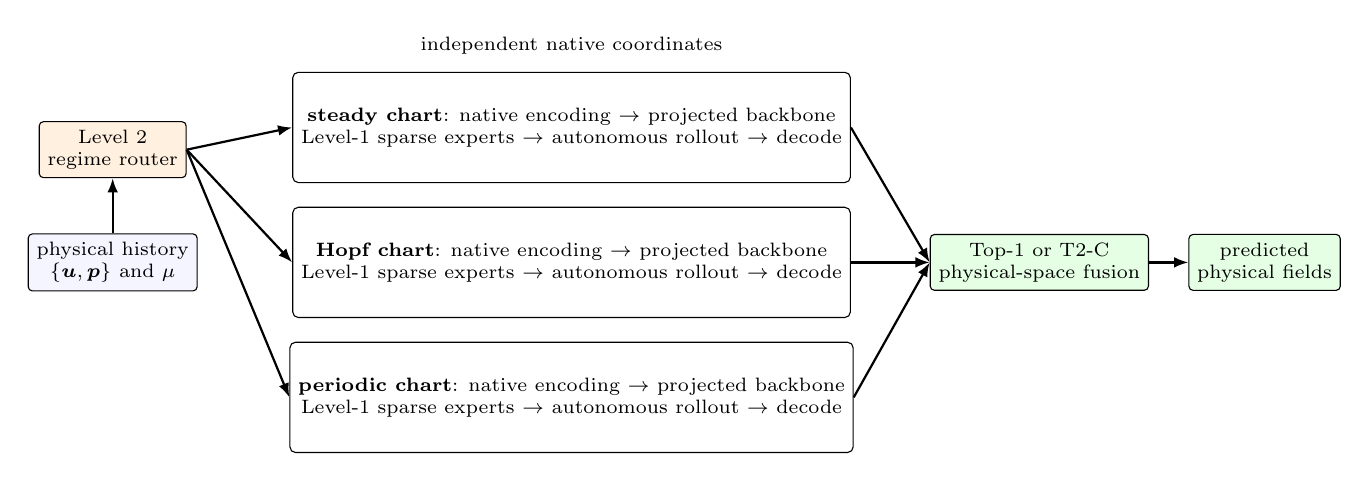
\begin{tikzpicture}[
  font=\scriptsize,
  node distance=4mm and 5mm,
  block/.style={draw,rounded corners=1.5pt,align=center,minimum height=7mm,inner sep=3pt,fill=blue!4},
  chart/.style={draw,rounded corners=2pt,align=center,minimum width=46mm,minimum height=14mm,inner sep=3pt},
  route/.style={draw,rounded corners=1.5pt,align=center,minimum height=7mm,inner sep=3pt,fill=orange!12},
  outputblock/.style={draw,rounded corners=1.5pt,align=center,minimum height=7mm,inner sep=3pt,fill=green!10},
  arrow/.style={-{Latex[length=1.8mm]},thick},
  soft/.style={-{Latex[length=1.5mm]},thin,dashed}
]
\node[block] (history) {physical history\\$\{\bm u,\bm p\}$ and $\mu$};
\node[route,above=7mm of history] (outer) {Level 2\\regime router};

\node[chart,right=12mm of history] (hopf) {\textbf{Hopf chart}: native encoding $\rightarrow$ projected backbone\\Level-1 sparse experts $\rightarrow$ autonomous rollout $\rightarrow$ decode};
\node[chart,above=3mm of hopf] (steady) {\textbf{steady chart}: native encoding $\rightarrow$ projected backbone\\Level-1 sparse experts $\rightarrow$ autonomous rollout $\rightarrow$ decode};
\node[chart,below=3mm of hopf] (periodic) {\textbf{periodic chart}: native encoding $\rightarrow$ projected backbone\\Level-1 sparse experts $\rightarrow$ autonomous rollout $\rightarrow$ decode};

\node[outputblock,right=10mm of hopf] (fusion) {Top-1 or T2-C\\physical-space fusion};
\node[outputblock,right=5mm of fusion] (prediction) {predicted\\physical fields};

\draw[arrow] (history) -- (outer);
\draw[arrow] (outer.east) -- (steady.west);
\draw[arrow] (outer.east) -- (hopf.west);
\draw[arrow] (outer.east) -- (periodic.west);
\draw[arrow] (steady.east) -- (fusion.west);
\draw[arrow] (hopf.east) -- (fusion.west);
\draw[arrow] (periodic.east) -- (fusion.west);
\draw[arrow] (fusion) -- (prediction);

\node[above=1mm of steady.north,align=center] {independent native coordinates};
\end{tikzpicture}
}
    \caption{Overview of RAL-MoE-ROM. The method uses sparse expert routing within each regime-local specialist and regime-level routing across complete local dynamical models. Adjacent specialists evolve independently in their native reduced coordinates and are combined only after reconstruction in the common physical space.}
    \label{fig:ral_overview}
\end{figure}

We evaluate RAL-MoE-ROM on three parametrized incompressible-flow systems spanning steady,
Hopf-onset, and periodic dynamics.
The experiments are designed to separate the roles of structured expert architecture,
projected physical dynamics, regime localization, and cross-regime routing.
Across the evaluated long-horizon rollouts, the local specialists remain accurate and
stable, while T2-C consistently improves the corresponding hard or single-specialist
prediction in the tested overlap regions.
The results also show that localization is not uniformly superior to a global model at every
parameter value; rather, its value emerges from combining local representation,
regime-specific dynamics, and adaptive cross-regime assembly.

\section{Related Work}

\paragraph{Projection and learned reduced dynamics.}
POD--Galerkin models obtain interpretable low-dimensional dynamics by projecting the governing equations onto a data-adapted basis \citep{sirovich1987,berkooz1993,benner2015}. Their main limitation is the influence of truncated scales and imperfect closure. Learned reduced models and neural operators provide flexible nonlinear approximations \citep{hesthaven2018,lu2021,kovachki2023}, while hybrid models retain a projected backbone and learn only unresolved corrections \citep{duraisamy2019,brunton2020,lee2020}. RAL-MoE-ROM follows the hybrid view but learns a conditionally sparse correction under closed-loop rollout rather than a single global residual map.

\paragraph{Local representations for parameterized dynamics.}
Local bases and clustered or manifold-based ROMs reduce the burden placed on a global representation \citep{amsallem2012,kaiser2014,li2021cluster,diaz2024}. These methods motivate our overlapping charts, but do not by themselves resolve how autonomous local models with unrelated coordinates should be assembled near regime boundaries. Our construction preserves each chart's own affine mean, basis, scaling, and operators, and defers coupling until after physical reconstruction.

\paragraph{Mixture-of-experts and conditional computation.}
MoE models route inputs among specialized predictors \citep{jacobs1991,jordan1994,shazeer2017,fedus2022}. Most architectures route experts acting in a shared feature space. In contrast, RAL-MoE-ROM uses two distinct routing levels: structured closure experts share one local chart, whereas the outer router selects complete autonomous specialists whose reduced coordinates are chart dependent. The latter are never averaged coefficientwise; adjacent predictions are fused only in the common physical space.

\section{RAL-MoE-ROM}
\label{sec:method}

We consider parameterized dynamics whose trajectories occupy qualitatively different regions of state space as the physical parameter $\mu$ varies. RAL-MoE-ROM separates representation, within-regime closure, and cross-regime assembly instead of forcing every trajectory into one latent coordinate system.

\subsection{Overlapping regime-local reduced charts}

Let $r\in\{S,H,P\}$ index steady, Hopf-onset, and periodic regimes, and let $\mathcal M_r$ denote overlapping parameter regions. Each chart has its own affine mean, velocity and pressure bases, scaling, and reduced operators. A physical state is encoded and reconstructed as
\begin{equation}
  \bm a^{(r)}=\bm\Phi_{u,r}^{\top}\bm W_u(\bm u-\bar{\bm u}_r),\qquad
  \widehat{\bm u}^{(r)}=\bar{\bm u}_r+\bm\Phi_{u,r}\bm a^{(r)},
  \label{eq:main_chart}
\end{equation}
with the analogous map for gauge-corrected pressure coefficients $\bm b^{(r)}$. Because these coordinates are constructed independently, components of $\bm a^{(r)}$ and $\bm a^{(s)}$ are not assumed to correspond when $r\neq s$. This is the reason cross-regime fusion is deferred to physical space.

\subsection{Physics--data specialists with structured sparse experts}

Projection supplies a regime-local dynamical backbone,
\begin{equation}
  \dot{\bm a}^{(r)}=
  \underbrace{\bm c_r+\bm A_r\bm a^{(r)}+
  \bm H_r:\bigl(\bm a^{(r)}\otimes\bm a^{(r)}\bigr)+
  \bm C^p_r\bm b^{(r)}}_{\mathcal F_r^{G}(\bm a^{(r)},\bm b^{(r)};\mu)}
  +\bm\rho^u_{\theta_r}(\bm\xi^{(r)}).
  \label{eq:main_specialist}
\end{equation}
The feature vector $\bm\xi^{(r)}$ contains standardized local coordinates, the projected right-hand side, the parameter, and a short state history. The learned correction is a channel-wise sparse MoE,
\begin{equation}
  \mathcal M^c_{\theta_r}(\bm\xi)=
  \omega^c_0 E^c_{0,g^\star}(\bm\xi)+
  \sum_{e\in\mathcal T^c}\omega^c_e E^c_{e,g^\star}(\bm\xi),
  \qquad
  E(\bm\xi)=N(\bm\xi)+W_{\rm lin}\bm\xi+
  \kappa W_o\bigl[(U^\top\bm\xi)\odot(V^\top\bm\xi)\bigr].
  \label{eq:main_inner_moe}
\end{equation}
The first routing decision selects a sparse expert group and the second selects experts within that group. The nonlinear, affine, and low-rank bilinear branches provide complementary correction structures without removing the explicit projected term. Pressure is reconstructed through a physics--data algebraic map rather than evolved as an unconstrained recurrent state; details are in Appendix~\ref{app:specialists}.

\subsection{Closed-loop autonomous training}

Each specialist is trained on rollout windows. Starting from encoded physical history, the numerical integrator repeatedly evaluates Eq.~\eqref{eq:main_specialist} on its own predictions. The loss aggregates velocity- and pressure-coordinate errors across the window, so the optimization sees the distribution shift produced by recursive use. All comparisons use the same held-out trajectories and the reported rollout horizons; exact splits are summarized in Table~\ref{tab:benchmark_summary} and Appendix~\ref{app:implementation}.

\subsection{Regime routing and physical-space T2-C fusion}

The outer E2 router maps the parameter and initial physical history to probabilities over admissible charts. Hard Top-1 prediction advances the largest-probability specialist. In a validated overlap only an adjacent pair is admissible ($S$--$H$ or $H$--$P$). Both specialists encode the same physical history in their native coordinates and then evolve independently. For reconstructed fields $\widehat{\bm q}^{(r)}$ and $\widehat{\bm q}^{(s)}$, T2-C predicts a window-conditioned convex weight and forms
\begin{equation}
  \widehat{\bm q}_{\rm T2C}(t)
  =\alpha\,\widehat{\bm q}^{(r)}(t)+(1-\alpha)\,\widehat{\bm q}^{(s)}(t),
  \qquad \alpha=\sigma\!\left(\operatorname{logit}(\bar\pi_r)+\Delta_\psi\right).
  \label{eq:main_t2c}
\end{equation}
Here $\bar\pi_r$ is the pair-normalized E2 probability and $\Delta_\psi$ is a learned correction from the shared physical input window. Fusion occurs after reconstruction and is not fed back into either local rollout. Admissibility is selected from validation support and should not be interpreted as a formal stability certificate.

\section{Experiments}
\label{sec:experiments}

We study three two-dimensional incompressible-flow systems with Reynolds number as the parameter: flow past a circular cylinder, flow past a centered square cylinder, and the fluidic pinball. Each dataset spans steady, Hopf-onset, and periodic behavior. Errors $E_u$ and $E_p$ are relative field errors in percent, averaged using the protocol of each benchmark; $E_{\rm joint}=E_u+E_p$ where reported. ``Divergent'' denotes a rollout that does not remain finite under the original evaluation rule. We preserve the numerical values and held-out partitions of the journal experiments.

\begin{table}[t]
\centering
\caption{Benchmark and held-out autonomous-rollout protocol. Entries list train/validation/test trajectories by local chart.}
\label{tab:benchmark_summary}
\small
\setlength{\tabcolsep}{3.2pt}
\begin{tabular}{lccc}
\toprule
Benchmark & $S$ chart & $H$ chart & $P$ chart \\
\midrule
Circular cylinder
 & 20.0--46.4; 14/2/4; $K{=}56$
 & 45.5--59.2; 29/2/3; $K{=}56$
 & 57.3--200; 53/6/4; $K{=}48$ \\
Centered square
 & 50--95.4; 60/5/4; $K{=}16$
 & 94--102; 23/6/5; $K{=}48$
 & 98.5--150; 27/6/4; $K{=}24$ \\
Fluidic pinball
 & 10--19; 37/8/7; $K{=}56$
 & 16.6--25; 39/8/7; $K{=}56$
 & 21.25--60; 47/9/9; $K{=}32$ \\
\bottomrule
\end{tabular}
\end{table}

\subsection{Do local specialists support long autonomous rollouts?}

On the circular cylinder, the proposed specialists remain finite across every evaluated regime. In the steady regime, their velocity-error range is $0.0330$--$0.1723\%$, compared with $0.0384$--$0.2995\%$ for a vanilla learned specialist and $0.0845$--$0.3404\%$ for the global model. In the Hopf regime the vanilla model is not evaluable, while RAL-MoE-ROM gives $E_u=0.0032$--$0.0288\%$ and $E_p=0.0355$--$0.4321\%$. In the periodic regime it improves the velocity-error range over vanilla from $1.0393$--$3.0836\%$ to $0.3809$--$1.3473\%$. Full pressure ranges and the data-only ablation are in Appendix~\ref{app:circular}.

The centered-square specialists transfer the construction to a different geometry and mesh. Aggregate held-out errors are $(E_u,E_p)=(1.5311,1.4583)\%$ for the steady chart, $(0.4387,0.4844)\%$ for Hopf, and $(0.9395,1.0921)\%$ for periodic flow. On fluidic pinball, the comparison in Table~\ref{tab:pinball_autonomous} shows that the learned specialist removes the divergent rollouts of the projected baseline in the steady and Hopf settings and substantially reduces joint error across all four evaluations. This is empirical long-horizon evidence under the tested distributions, not a guarantee of stability outside them.

\begin{table}[t]
\centering
\caption{Fluidic-pinball autonomous prediction. Errors are percentages; ``div.'' counts divergent evaluation windows.}
\label{tab:pinball_autonomous}
\small
\setlength{\tabcolsep}{3.5pt}
\begin{tabular}{llrrrr}
\toprule
Regime ($K$) & Model & $E_u$ & $E_p$ & $E_{\rm joint}$ & div. \\
\midrule
Steady (56) & POD--Galerkin & -- & -- & -- & 448/448 \\
            & RAL-MoE-ROM & 0.2247 & 0.7593 & 0.9840 & 0 \\
Hopf (56)   & POD--Galerkin & 0.4378 & 48.50 & 48.94 & 141/320 \\
            & RAL-MoE-ROM & 0.0995 & 1.986 & 2.085 & 0 \\
Periodic (32) & POD--Galerkin & 1.641 & 41.56 & 43.20 & 0 \\
            & RAL-MoE-ROM & 0.2897 & 0.5518 & 0.8415 & 0 \\
Periodic core (56) & POD--Galerkin & 2.555 & 39.36 & 41.91 & 0 \\
            & RAL-MoE-ROM & 0.6222 & 1.050 & 1.672 & 0 \\
\bottomrule
\end{tabular}
\end{table}

\subsection{Does learned physical-space fusion improve overlap prediction?}

Table~\ref{tab:routing_fusion} separates hard routing from field-space combination on the centered-square benchmark. T2-C improves E2 Top-1 in both overlaps and is close to the a posteriori window-wise convex oracle. Equal weights and direct E2-probability weights do not reproduce the gain, indicating that the improvement is not a generic consequence of averaging. At $Re=95.1$, T2-C reduces joint error from $1.7140\%$ to $1.1827\%$; at $Re=100.5$, it reduces $2.6485\%$ to $0.8571\%$. Figure~\ref{fig:square_overlap} shows the corresponding physical fields and velocity-error maps. The complete parameter-wise table and fluidic-pinball overlap study appear in Appendices~\ref{app:square} and \ref{app:pinball}.

\begin{table}[t]
\centering
\caption{Centered-square routing and fusion at $K=24$. Lower is better.}
\label{tab:routing_fusion}
\small
\setlength{\tabcolsep}{4pt}
\begin{tabular}{llrrr}
\toprule
Overlap & Predictor & $E_u$ & $E_p$ & $E_{\rm joint}$ \\
\midrule
$S$--$H$ & E2 Top-1 & 0.4942 & 1.2356 & 1.7298 \\
          & Equal blend & 1.3644 & 1.6677 & 3.0321 \\
          & E2-probability blend & 0.7898 & 1.3949 & 2.1847 \\
          & T2-C & \textbf{0.4615} & 0.7343 & \textbf{1.1958} \\
          & Convex oracle & 0.4659 & \textbf{0.7183} & 1.1842 \\
\midrule
$H$--$P$ & E2 Top-1 & 0.7422 & 1.1052 & 1.8473 \\
          & Equal blend & 0.6077 & 1.0069 & 1.6146 \\
          & E2-probability blend & 0.6154 & 1.0464 & 1.6618 \\
          & T2-C & 0.4509 & 0.3956 & 0.8465 \\
          & Convex oracle & \textbf{0.4479} & \textbf{0.3905} & \textbf{0.8384} \\
\bottomrule
\end{tabular}
\end{table}

\begin{figure}[t]
\centering
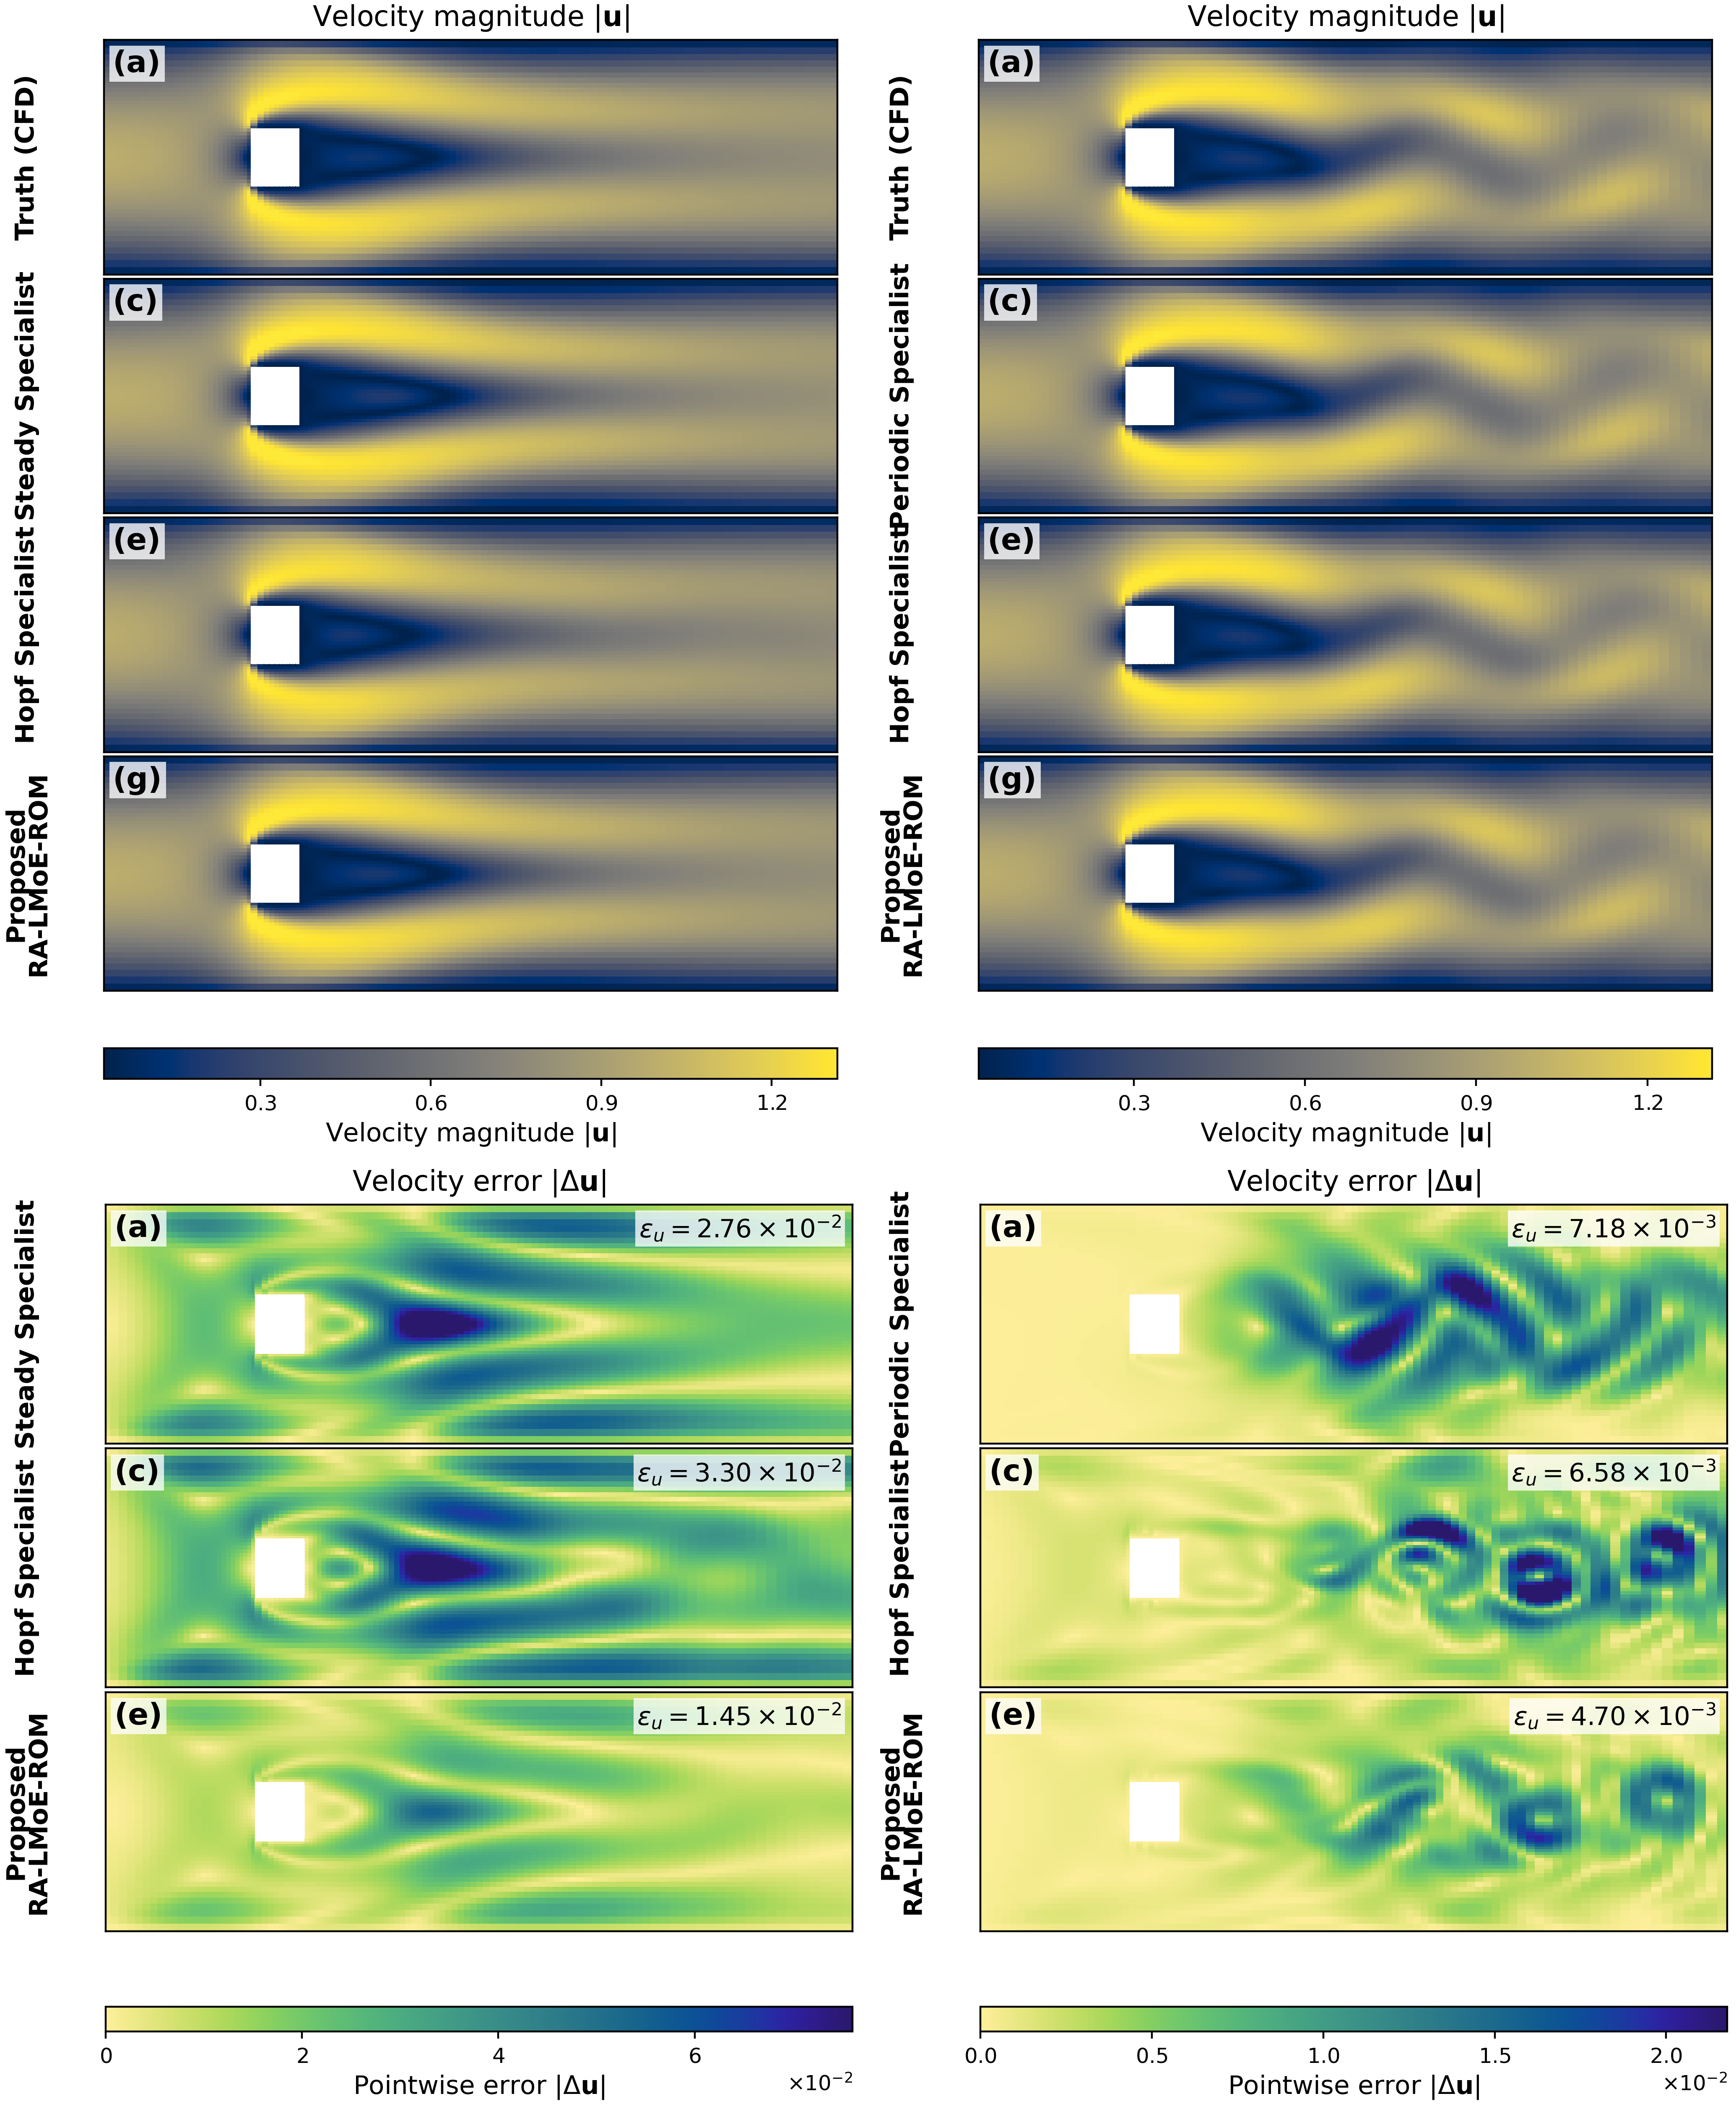
\includegraphics[width=\linewidth]{figures/square_overlap_compact.png}
\caption{Centered-square overlap predictions. Left: $S$--$H$ at $Re=95.1$; right: $H$--$P$ at $Re=100.5$. The upper panels compare CFD, the two adjacent specialists, and RAL-MoE-ROM using velocity magnitude. The lower panels show the corresponding absolute velocity errors. The composite crops only the velocity columns from the original full velocity--pressure panels and preserves their native raster pixels.}
\label{fig:square_overlap}
\end{figure}

\subsection{What contributes to the result?}

The original ablations isolate four effects. Removing the projected backbone produces the data-only degradation visible on circular-cylinder rollouts; replacing localized specialists with one global model sacrifices regime-specific accuracy, although the global model can remain competitive at individual parameters; replacing structured sparse experts with the vanilla learned correction widens long-horizon errors and fails in the evaluated Hopf case; and replacing T2-C with Top-1, equal, or raw-probability fusion worsens overlap prediction. Together these results support the architectural decomposition rather than a claim that any single component is uniformly dominant.

\section{Limitations}

The regime cover and admissible adjacency graph are selected using validation support; the method does not discover arbitrary bifurcation structure or certify unseen transitions. T2-C is evaluated only between adjacent specialists, and its convex physical-space fusion may be insufficient when more than two regimes interact or when conserved quantities require a constrained assembly rule. The reported evidence concerns two-dimensional incompressible flows and empirical finite-horizon behavior. It does not establish provable stability, conservation, or accuracy outside the sampled parameter ranges. Finally, maintaining multiple local bases, projected operators, and specialists increases training and model-management cost relative to a single global ROM.

\section{Conclusion}

RAL-MoE-ROM casts broad-parameter reduced dynamics as a two-level mixture-of-experts problem. Structured sparse experts learn unresolved dynamics inside each physics--data specialist, while an outer router selects or combines complete local models. Keeping the local coordinates independent and coupling only reconstructed physical fields avoids interpolation between incompatible modal states. Across the three evaluated flow systems, the specialists support accurate autonomous rollout and T2-C improves prediction in the tested transition regions. The results motivate extensions that learn the regime cover, impose physical constraints on field-space fusion, and evaluate the hierarchy on higher-dimensional and non-fluid dynamical systems.


\subsubsection*{Reproducibility statement}
The main text reports the data splits, rollout horizons, reduced dimensions, baselines, and evaluation metrics needed to interpret the results. Appendix~\ref{app:implementation} documents the local-coordinate construction, specialist architecture, routing procedure, and additional benchmark results. The anonymous supplementary material will include the training and evaluation configuration required to reproduce the reported tables.

\subsubsection*{AI use statement}
\textbf{TODO: authors to complete final disclosure.}

\bibliography{references,legacy_references}
\bibliographystyle{iclr2027_conference}

\appendix
\section{Reproducibility and implementation details}
\label{app:implementation}

\paragraph{Evaluation protocol.}
All headline results use trajectories held out by Reynolds number. Each local specialist is fitted only on its stated training split, model selection uses the validation split, and the test split is retained for the reported autonomous rollouts. The reduced model is initialized from the same available physical history used by the original experiments and is then advanced recursively with fourth-order Runge--Kutta integration. No reference state from inside a prediction window is injected after initialization.

\paragraph{Local dimensions.}
For the circular cylinder, all three charts use $r_u=r_p=32$. For the centered square, $(r_u,r_p)$ equals $(5,4)$, $(11,11)$, and $(28,26)$ for the steady, Hopf, and periodic charts. For fluidic pinball the corresponding dimensions are $(4,3)$, $(5,5)$, and $(17,16)$. The full-order datasets contain 120 centered-square trajectories over $Re\in[50,150]$ and 131 fluidic-pinball trajectories over $Re\in[10,60]$; the centered-square finite-volume mesh contains 9,400 cells and uses snapshot spacing $\Delta t=4$.

\paragraph{Model selection and reporting.}
The outer regime graph permits only adjacent $S$--$H$ and $H$--$P$ pairs. Hyperparameters, rollout windows, and routing choices are selected on validation data. Reported percentages are copied from the original experiment tables without recomputation. For anonymity, repository locations, author names, institutions, and machine-specific paths are excluded from the submission artifact.

\paragraph{Artifact checklist.}
The final anonymous supplement should contain preprocessing code, train/validation/test parameter lists, local means and basis construction, projected operators, trained configurations, random seeds, rollout evaluation, and table-generation scripts. The present conversion directory preserves an untouched PDF and source snapshot for author-side verification, but those identity-bearing files must not be uploaded with the anonymous submission.

\section{Regime-local projection details}
\label{app:rom}

For each regime $r$, snapshots are centered with a chart-specific affine mean. Velocity POD uses the discrete kinetic-energy inner product $\langle\bm x,\bm y\rangle_{W_u}=\bm x^\top W_u\bm y$; pressure uses the corresponding cell-area weighting. The bases satisfy $\Phi_{u,r}^\top W_u\Phi_{u,r}=I$ and $\Phi_{p,r}^\top W_p\Phi_{p,r}=I$. Pressure snapshots are gauge corrected before basis construction, so additive pressure constants do not enter either training or evaluation.

Writing
\begin{equation}
  \bm u\approx\bar{\bm u}_r+\Phi_{u,r}\bm a^{(r)},\qquad
  \bm p\approx\bar{\bm p}_r+\Phi_{p,r}\bm b^{(r)},
\end{equation}
and projecting the semi-discrete incompressible momentum equation gives
\begin{equation}
  \dot a_i^{(r)}=c_{r,i}+\sum_j A_{r,ij}a_j^{(r)}
  +\sum_{j,k}H_{r,ijk}a_j^{(r)}a_k^{(r)}
  +\sum_j C^p_{r,ij}b_j^{(r)}.
\end{equation}
The constant, linear, quadratic, and pressure-coupling tensors are computed separately in every chart. Pressure coefficients are obtained by projecting the pressure--Poisson relation and combining that physical estimate with a learned algebraic correction. This construction preserves the projected vector field as the explicit backbone in Eq.~\eqref{eq:main_specialist}; the MoE models the discrepancy rather than replacing the entire reduced dynamics.

The affine offsets, bases, coordinates, and tensors are chart dependent. Even if two charts use the same reduced dimension, their coefficient vectors are therefore not interchangeable. This noncommensurability is structural and motivates the physical-space assembly in Appendix~\ref{app:routing}.

\section{Specialist architecture and closed-loop objective}
\label{app:specialists}

Each specialist receives standardized velocity and pressure coordinates, the Galerkin right-hand side, the physical parameter, and two preceding local states. Separate channel routers produce velocity and pressure corrections. A first sparse decision selects an expert group and a second decision activates a small set of experts within the group. Every expert combines a nonlinear branch, an affine skip, and a low-rank bilinear interaction,
\begin{equation}
 E(\xi)=N(\xi)+W_{\rm lin}\xi+\kappa W_o[(U^\top\xi)\odot(V^\top\xi)].
\end{equation}
The selected expert outputs are weighted and added to the projected dynamics. The pressure path combines a projected pressure--Poisson estimate and a data-driven algebraic map using a componentwise gate.

For a rollout window of length $K$, the training objective evaluates predictions generated recursively from the model's own previous states,
\begin{equation}
 \mathcal L_{\rm roll}=\frac{1}{K}\sum_{k=1}^{K}
 \left(\lambda_u\|\widehat{\bm a}_k-\bm a_k\|_2^2+
       \lambda_p\|\widehat{\bm b}_k-\bm b_k\|_2^2\right)
 +\lambda_{\rm route}\mathcal R_{\rm route}.
\end{equation}
The routing regularizer promotes sparse use without forcing every sample through the same branch. The important experimental distinction from a one-step learner is that the state supplied at step $k+1$ is the model prediction at step $k$.

\section{Outer routing and T2-C details}
\label{app:routing}

The E2 router produces chart probabilities from the parameter and initial physical history. Validation support defines the admissible set and the adjacency graph $S$--$H$--$P$. Top-1 advances one complete specialist. For an admissible pair $(r,s)$, pair probabilities are normalized as
\begin{equation}
 \bar\pi_r=\frac{\pi_r}{\pi_r+\pi_s},\qquad
 \bar\pi_s=1-\bar\pi_r.
\end{equation}
T2-C initializes both specialists from the same physical observations, encodes them separately, and performs two independent autonomous rollouts. A correction network predicts a bounded logit offset, producing $\alpha=\sigma(\operatorname{logit}\bar\pi_r+\Delta_\psi)$. Velocity and gauge-corrected pressure fields are reconstructed in the common mesh before the convex combination is applied. The fused field is used for output only and never projected back into either rollout.

The equal blend fixes $\alpha=1/2$; the probability blend sets $\alpha=\bar\pi_r$; and the convex oracle selects the best weight a posteriori for each evaluation window. The oracle is a reference, not a deployable method. Close agreement between T2-C and the oracle therefore quantifies how much of the pair's available complementarity the learned correction captures.

\section{Circular-cylinder results}
\label{app:circular}

Table~\ref{tab:circular_full} reports the original range over held-out long-horizon rollouts. ``N/E'' denotes the original not-evaluable entry.

\begin{table}[h]
\centering
\caption{Circular-cylinder long-horizon error ranges (\%).}
\label{tab:circular_full}
\small
\setlength{\tabcolsep}{4pt}
\begin{tabular}{llcc}
\toprule
Regime & Model & $E_u$ & $E_p$ \\
\midrule
Steady & RAL-MoE-ROM & 0.0330--0.1723 & 0.2500--1.3249 \\
 & Vanilla & 0.0384--0.2995 & 2.2163--18.5603 \\
 & Data only & 0.1637--0.5122 & 4751.1025--27275.4645 \\
 & Global & 0.0845--0.3404 & 1.5226--7.4363 \\
\midrule
Hopf & RAL-MoE-ROM & 0.0032--0.0288 & 0.0355--0.4321 \\
 & Vanilla & N/E & N/E \\
 & Data only & 0.1260--0.3880 & 1280.2811--1524.5949 \\
 & Global & 0.0110--0.0268 & 0.0560--0.2882 \\
\midrule
Periodic & RAL-MoE-ROM & 0.3809--1.3473 & 1.6825--5.9601 \\
 & Vanilla & 1.0393--3.0836 & 3.9659--13.3257 \\
 & Data only & 0.7854--1.8677 & 2.2511--10.8189 \\
 & Global & 0.5873--1.1726 & 2.1896--6.3566 \\
\bottomrule
\end{tabular}
\end{table}

In the $S$--$H$ overlap, E2 Top-1 gives $E_u=0.0357$--$0.0410\%$ and $E_p=1.6746$--$1.9028\%$. T2-C reduces these ranges to $0.0148$--$0.0355\%$ and $0.7387$--$1.7212\%$, with mean steady weight spanning $0.0861$--$0.9987$. The global model yields $E_u=0.0851$--$0.0953\%$ and $E_p=1.9517$--$2.3106\%$ on the same overlap evaluation.

\section{Centered-square results}
\label{app:square}

\begin{table}[h]
\centering
\caption{Parameter-wise centered-square routing and T2-C results at $K=24$. The mean weight is the steady weight for $S$--$H$ and the periodic weight for $H$--$P$.}
\label{tab:square_parameter}
\small
\setlength{\tabcolsep}{3.5pt}
\begin{tabular}{lrlrrrr}
\toprule
Overlap & $Re$ & E2 choice & $\bar\alpha$ & E2 joint & T2-C joint & reduction \\
\midrule
$S$--$H$ & 95.1 & Hopf & 0.0967 & 1.7140 & 1.1827 & 31.00\% \\
$S$--$H$ & 95.3 & Hopf & 0.0971 & 1.7456 & 1.2090 & 30.74\% \\
$H$--$P$ & 100.5 & Hopf & 0.5870 & 2.6485 & 0.8571 & 67.64\% \\
$H$--$P$ & 102.0 & Periodic & 0.7094 & 1.0462 & 0.8360 & 20.09\% \\
\bottomrule
\end{tabular}
\end{table}

The aggregate local-specialist errors are $(E_u,E_p)=(1.5311,1.4583)\%$ for steady flow, $(0.4387,0.4844)\%$ for Hopf-onset flow, and $(0.9395,1.0921)\%$ for periodic flow. On the aggregate $S$--$H$ evaluation, the steady and Hopf specialists have joint errors $4.8426\%$ and $1.7298\%$; on $H$--$P$, the periodic and Hopf specialists give $1.2079\%$ and $2.8718\%$. These results show why the best local choice can change between overlaps and why a corrected convex assembly is useful.

For auditability, the uncropped velocity--pressure and pointwise-error rasters used to construct Fig.~\ref{fig:square_overlap} are retained under \texttt{figures/original}. They should be included in supplementary material only if the final anonymous package needs the full pressure panels.

\section{Fluidic-pinball results}
\label{app:pinball}

The fluidic-pinball dataset contains 131 trajectories over $Re\in[10,60]$, with 94/19/18 train/validation/test trajectories overall. A POD--DeepONet one-step baseline gives $E_u=1.5921\%$ and $E_p=23.3447\%$ on 4,228 held-out input--output pairs, but only 1 of 28 held-out trajectories remains finite under recursive rollout. This contrast motivates evaluation under autonomous use rather than one-step accuracy alone.

\begin{table}[h]
\centering
\caption{Fluidic-pinball overlap joint errors (\%).}
\label{tab:pinball_overlap}
\small
\setlength{\tabcolsep}{3.5pt}
\begin{tabular}{lrccccc}
\toprule
Overlap & $K$ & primary & adjacent & E2-prob. & T2-C & oracle \\
\midrule
$S$--$H$ & 24 & 0.6014 & 3.1925 & 1.7511 & 0.5897 & 0.5889 \\
$S$--$H$ & 56 & 0.6927 & 3.1193 & 1.7714 & 0.6767 & 0.6763 \\
$H$--$P$ & 24 & 0.0990 & 0.5146 & 0.2972 & 0.0945 & 0.0928 \\
$H$--$P$ & 56 & 0.1028 & 0.5346 & 0.3085 & 0.0978 & 0.0955 \\
\bottomrule
\end{tabular}
\end{table}

T2-C improves the primary single-specialist prediction in all four overlap evaluations and remains close to the window-wise convex oracle. The result is consistent across the short and long rollout horizons shown here.


\end{document}
